\subsection{The Current State of ECDAR}\label{sub:the-current-state-of-ecdar} %This was written quite fastly ;)
This section will go over the ECDAR tool, to further illustrate the intent of ECDAR and how far it has been developed. The GUI of ECDAR 2.3.3 can be seen in \autoref{fig:ECDAR-gui}.

The GUI is split up into three vertical panes, as seen in \autoref{fig:ECDAR-gui}. The different components in the project are listed in the project pane to the left, the currently selected component is shown in the editor pane in the middle, and the queries are found in the query pane to the right.
The GUI also has a top bar, from where it is possible to open a project, hide panes, choose engine options, and more.  
Additionally, the GUI has a bar in the bottom of the view. Here, errors and warnings are supposed to be displayed.

\begin{figure}[H]
    \centering
    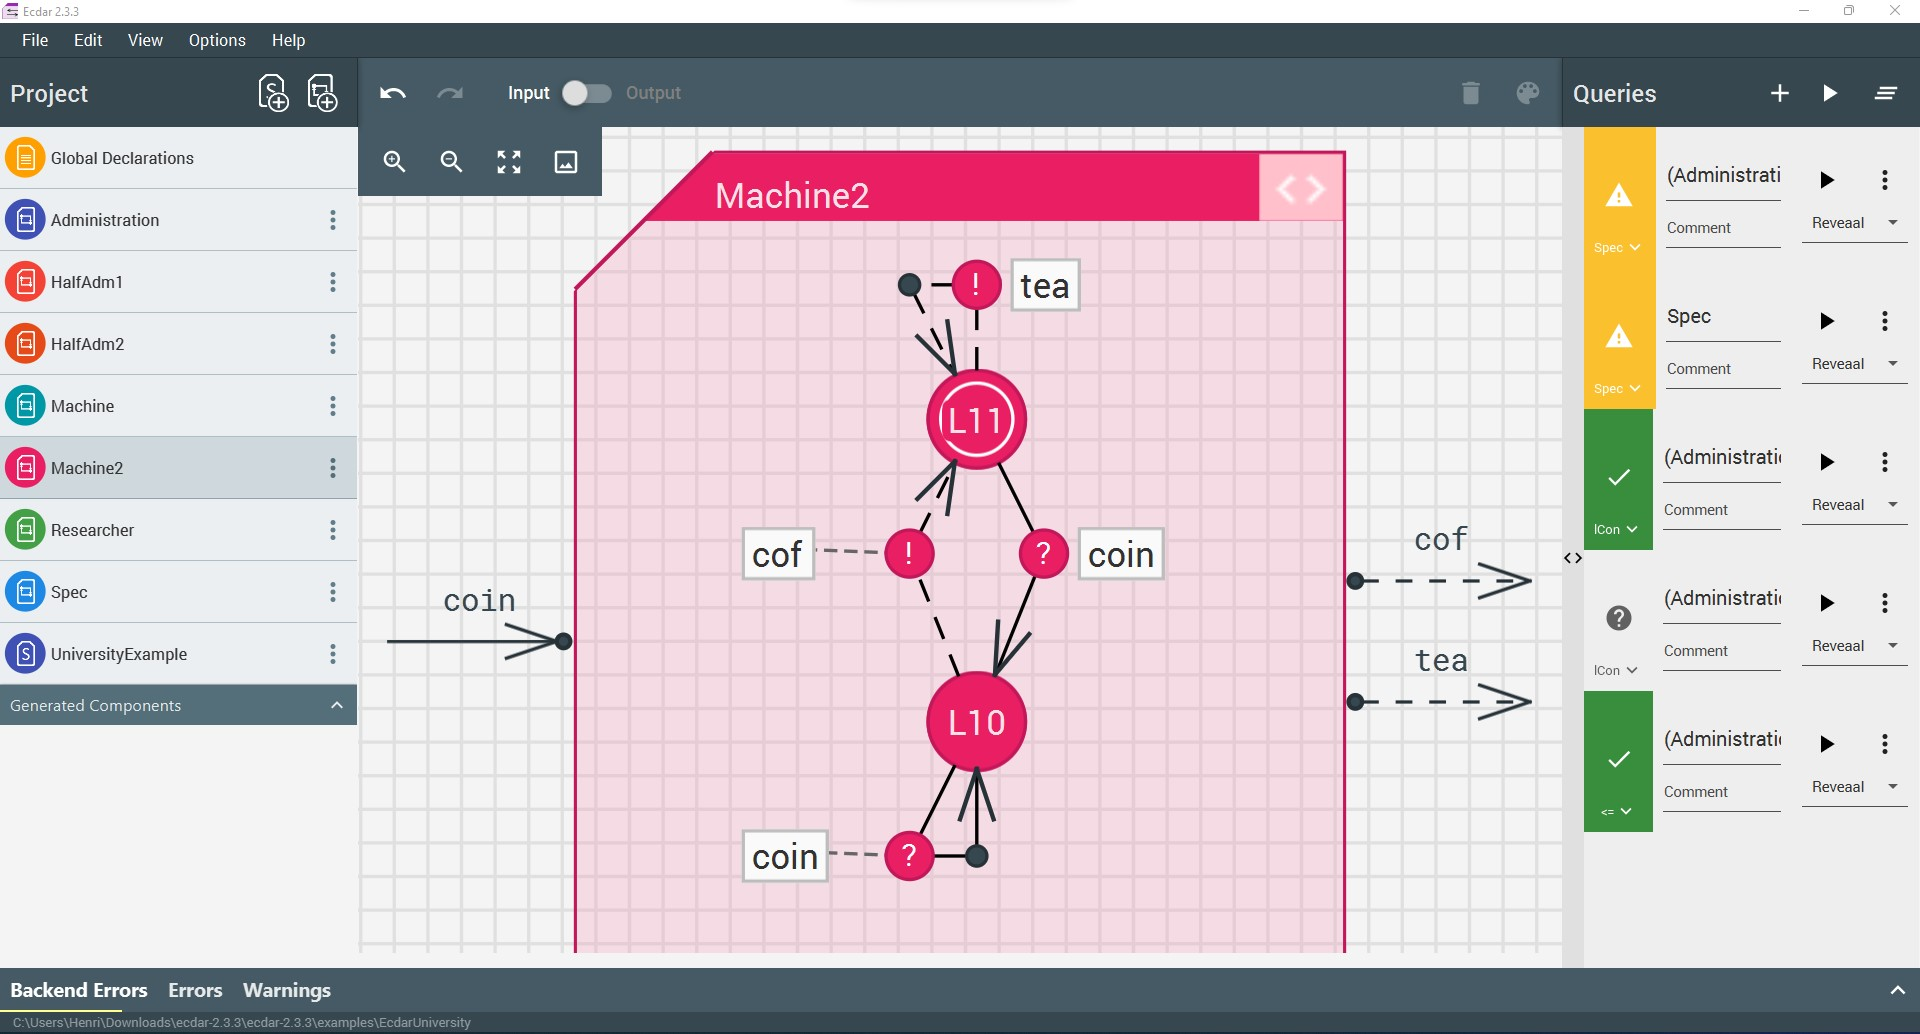
\includegraphics[width=1\textwidth]{common/figures/ecdar-overview.jpg}
    \caption{A screenshot of the ECDAR GUI of the latest version (ECDAR 2.3.3 released on 2022-09-08) \cite{ECDARNET_releasenotes}.}
    \label{fig:ECDAR-gui}
\end{figure}

\subsubsection{Project Pane}
The project pane has a header containing two buttons for creating new components and systems. The components are listed alphabetically just below this header. 
In the bottom of the pane, there is a section for automatically generated components.

\subsubsection{Editor Pane}
In \autoref{fig:ECDAR-gui}, the component \textit{Machine2} is selected. Therefore, it is shown in the editor pane. The editor pane can display one or four components at a time.
In the editor pane, it is possible to modify the components, e.g., by adding and removing transitions and locations.

%evt tilføj et teori afsnit 

\textit{Machine2} is a model of a coffee machine. The accepted input is shown on the left side of the component as a solid arrow pointing towards the component, here the input is . On the right side, the output from the coffee machine is illustrated with dashed arrows pointing away from the component. 
Inside the component, the model is composed of locations in the shape of big circles, and transitions marked by arrows between the locations. The initial location, \texttt{L11}, is marked by a white circle around the . 


It takes \texttt{coin} as input, since the arrow is solid, and the automaton outputs \texttt{cof} and \texttt{tea}, as shown by the dashed arrows on the right side of the automaton.
Inside the red box, the \texttt{L11} location is marked as the start state, which is indicated by the circle.
A solid arrow through a small circle with a question mark represents an output. 
Likewise, if the arrow is dashed and the small circle contains an exclamation mark, it represents an input.
This concludes the possibilities regarding input and output.

\autoref{fig:ECDAR-guard} contains an automaton which uses time as well as input and output.
This is done by using a clock, represented as the variable y.
\begin{figure}[H]
    \centering
    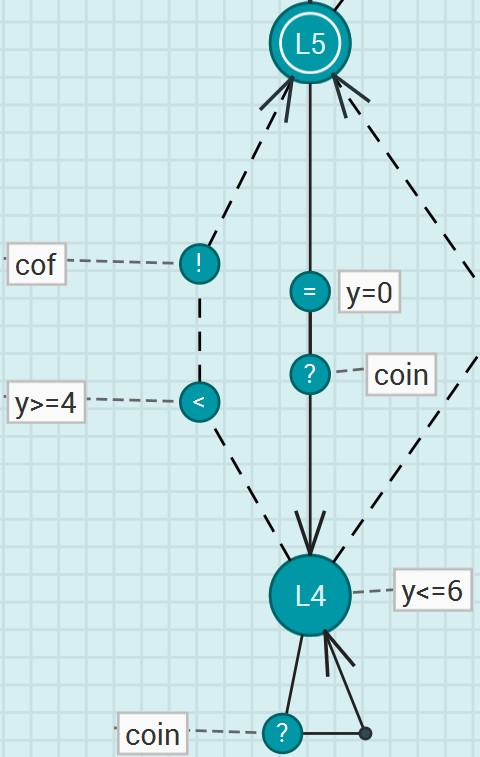
\includegraphics[width=0.3\textwidth]{common/figures/ecdar-guards.jpg}
    \caption{A screenshot of an automaton with a guard and an invariant.}
    \label{fig:ECDAR-guard}
\end{figure}

The transition with the small circle containing the assignment is an \textit{update} that resets the clock.
The small circle containing a "$<$"-sign is a type of \textit{guard}, which can be thought of as a restriction that must be satisfied in order to take this action/transition.
Finally the \texttt{L4}-location contains an \textit{invariant} \texttt{y<=6}, which must be satisfied. 
In this case, it means the automaton cannot be in the location if the clock value exceeds the value of 6.


\subsubsection{Query Pane}
The rightmost panel displays the queries to be performed. 
Queries are sent to one of the two engines, which can be selected in the drop-down menu, one of which can be seen in the bottom-right corner of \autoref{fig:ECDAR-queries-panel}. 
\begin{figure}[H]
    \centering
    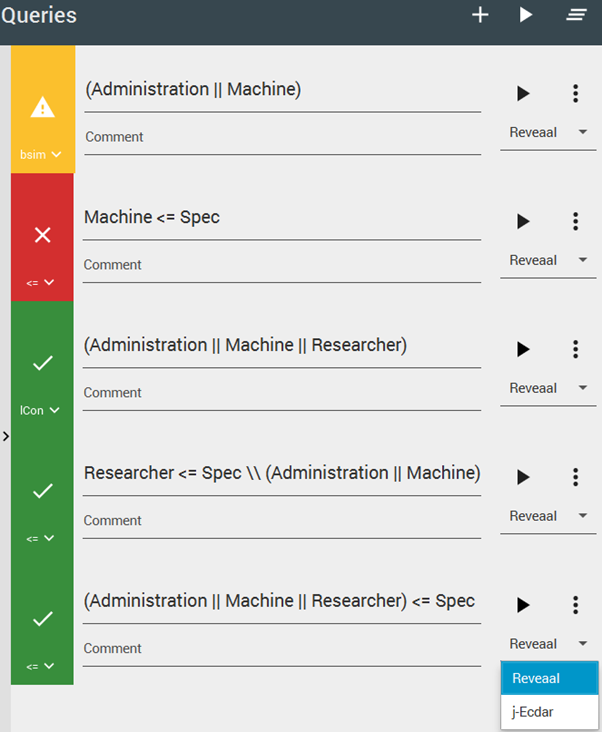
\includegraphics[width=0.6\textwidth]{common/figures/right-panel.png}
    \caption{A screenshot of the right panel of the GUI, which displays the queries.}
    \label{fig:ECDAR-queries-panel}
\end{figure}
To send the queries to be checked, the button with the \say{play} icon must be pressed.
Afterwards the result can be viewed on the left side of the panel in the form of an icon and a color. 
The result of the query in the top of \autoref{fig:ECDAR-queries-panel} is an error, which means the engine could not perform the query. 
An error message can be seen by placing the mouse over the icon, which can be used to troubleshoot why this error occurred.
The "Machine$<=$Spec" query was performed, but the result was false, which means the \texttt{Machine} model does not refine the specification named \texttt{Spec}, as illustrated by the red color and a cross.
The rest of the queries were performed without errors, and all proved true. 
The text boxes use a special syntax to specify a combination of models, operators, and specifications to be checked.

\begin{figure}[H]
    \centering
    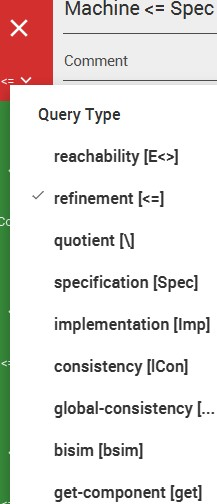
\includegraphics[width=0.25\textwidth]{common/figures/check-type.jpg}
    \caption{A screenshot of drop-down menu with the query types.}
    \label{fig:ECDAR-query-types}
\end{figure}

The type of the query to be performed is chosen in the drop-down menu underneath the icons. 
The drop-down menu with the types of queries that can be chosen, can be seen in \autoref{fig:ECDAR-query-types}.


